  
\documentclass[pldi]{sigplanconf-pldi15}

%
% the following standard packages may be helpful, but are not required
%
\usepackage{SIunits}            % typset units correctly
%\usepackage{courier}            % standard fixed width font
\usepackage{pdfpages}
\usepackage[scaled]{helvet} % see www.ctan.org/get/macros/latex/required/psnfss/psnfss2e.pdf
\usepackage{url}                  % format URLs
\usepackage{listings}          % format code
\usepackage{enumitem}      % adjust spacing in enums
\usepackage[colorlinks=true,allcolors=blue,breaklinks,draft=false]{hyperref}   % hyperlinks, including DOIs and URLs in bibliography
% known bug: http://tex.stackexchange.com/questions/1522/pdfendlink-ended-up-in-different-nesting-level-than-pdfstartlink
\newcommand{\doi}[1]{doi:~\href{http://dx.doi.org/#1}{\Hurl{#1}}}   % print a hyperlinked DOI

\lstset{
  %frame=tb,
  language=Haskell,
  aboveskip=3mm,
  belowskip=3mm,
  showstringspaces=false,
  columns=flexible,
  basicstyle={\footnotesize\ttfamily},
  numbers=none,
  breaklines=true,
  breakatwhitespace=true,
  tabsize=2
}

\begin{document}

%
% any author declaration will be ignored  when using 'plid' option (for double blind review)
%

\title{Pollstr: An EDSL for Easy Survey Creation}
\authorinfo{Jayme Woogerd} {jayme.woogerd@tufts.edu}

\maketitle
\begin{abstract}
Statistical surveys are an important means of data collection in many 
quantitative research fields including economics, psychology, sociology, and health.
This paper presents Pollstr, a programming language embedded in Haskell for 
specifying and generating statistical surveys. Pollstr makes it easy for 
domain experts with relatively little programming knowledge to declaratively 
specify a survey and generate it multiple media forms.
\end{abstract}

\section{Introduction}

Investigators in quantitative research fields commonly use statistical surveys, administered 
to a sample of individuals, to gather information and make statistical 
inferences about the populations they are studying. Statistical
surveys are an important means of data collection in many domains including
economics, psychology, sociology, and health. Surveys can be administered in a 
variety of modes, the most common of which include telephone, mail, online, 
and in-person \cite{scheuren}.

Naturally, with the rise of 
Web technologies and the ubiquity of fast Internet access, the use of online
surveys has grown, and with it an ecosystem of software tools and Web
services for creating and disseminating surveys online. Two well known examples
of such tools are Qualtrics and Survey Monkey, both of which provide users with 
survey templates, integration with email services, and some features for 
statistical analysis and reporting. These tools are designed to be easy to use 
for non-programmers, however as with any software, the user is limited to the
features provided by the software implementer. Furthermore, a researcher 
interested in administering the same survey via multiple modes (e.g. online and 
in-person) would have to duplicate efforts, as these services are designed for 
online deployment only.

As an alternative, this paper presents Pollstr, a programming language 
embedded in Haskell for specifying and generating statistical surveys. Given the
domain and issues stated above, Pollstr is designed to support the following
key goals:
\paragraph{Small, simple, and easy to learn for non-programmers}
The intended users of Pollstr are domain experts in quantitative research 
fields in which surveys are a major means of data collection, e.g. economics or
education. Such researchers generally have knowledge of survey design and 
analysis methods, but may have little or no programming experience. Therefore,
Pollstr is designed to be simple and approachable to the programming novice who
is willing to leave the comforts of a commercial online survey generator.

\paragraph{Declare once, deploy in multiple modes}
A researcher may wish to deploy the same survey via multiple modes -- for 
example, in areas of the world where some members of the population have Internet 
access and others do not, it may make sense to have both a print and an online
version of a survey. To ease the burden on the survey designer, Pollstr provides 
for the generation of multiple artifacts from a single survey declaration, 
i.e. supports both print-based and Web-based deployment interfaces.

\paragraph{Use the power and flexibility of a programming language}
Using a programming language to create surveys has the advantage of opening the 
domain to powerful and fundamental programming concepts: abstraction, code reuse,
and single points of truth. Users should be able to take advantage of these ideas
to make surveys that are easier to write and maintain. Additionally, a
language opens the possibility for greater flexibility and user-defined extension. \\

The remainder of this paper is structured as follows: Section \ref{sec:design} 
describes the current language features of Pollstr and illustrates them with a short
example. Implementation details are presented in Section \ref{sec:implemenation} and 
Section \ref{sec:evaluation} discusses evaluation methods. Section \ref{sec:related}
briefly discusses a related project. Finally, Section \ref{sec:future}
lists ideas for future work, including domain-specific tools and libraries that 
would be useful.

\section{Language Design}\label{sec:design}

In broad terms, a survey designer will want to: 1) create a survey by 
writing questions and responses, 2) generate and deploy the survey via one or 
more modes, and 3) perform statistical analysis on the results. In its current 
construction, Pollstr's set of features is just large enough to write and 
generate simple surveys. Programmers can specify common survey structures, 
write survey questions of a single response type (single-choice, in which a single 
response may be checked), and render the survey in two formats: in print via 
LaTeX and on the Web via JSON.

In addition, Pollstr includes a simple control flow construct for conditional 
question skipping, a common survey feature. Conditional skips allow questions
to be either presented or omitted, depending on the subject's response to a previous
question. In summary, Pollstr's features include:

\begin{enumerate}
\item A simple, declarative concrete syntax for specifying surveys, metadata 
(title, author, etc), sections, questions, and responses
\item Variable binding for questions and responses 
\item A simple construct for skip logic
\item Multiple artifact generation: LaTeX for print-based rendering and JSON 
for Web-based rendering
\end{enumerate}

\begin{figure}
\begin{lstlisting}
Response ff = ["Fact", "Fiction"]

Survey Demo:
    Title: "An Example Survey"
    Author: "Jayme Woogerd"
    Description: "This Pollstr program demonstrates key features, such as bound variables, sections, and skip logic. Enjoy!"

    Section First: "Would You Rather?"
        Q1: "Would you rather only be able to speak in Perl or only be able to talk when others are talking about Perl? "
            ["Speak in Perl",
             "Talk when others are talking about Perl"]
            skipTo(Q5, ["Speak in Perl"])

        Q4: "Would you rather be a garbage collector or a nomad monad?"
            ["Garbage collector!",
             "Nomad monad!"]

    Section Second: "Fact or Fiction"
        Q5: "Fact or Fiction: Bruce Molay has a black belt in karate." ff

        Q11: "Fact or Fiction: Sam Guyer is is a licensed airplane pilot." ff
\end{lstlisting}
  \caption{Example Pollstr survey}
  \label{fig:code}
  \end{figure}

The program in Figure \ref{fig:code} has all the elements of a complete Pollstr program: variable
binding, skip logic, and declarations for surveys, metadata, sections, 
and survey items. This example shows how the declarative forms for surveys and 
sections make for a a clear, structured program that reads very much like English 
text. Likewise, its is straightforward to declare optional metadata, which 
includes the title of the survey, the author, and a description of the survey.

The meat of the survey are the survey items, which the programmer declares 
with a "Q"followed by a unique alphanumeric identifier (in Figure \ref{fig:code}, all 
identifiers are numeric). Each survey item includes a question, list of 
response values, and optionally a \mono{skipTo} construct to specify any 
conditional skip directives. Skips resemble a traditional function call with
two parameters: a "destination" item and the set of response values 
for which to execute the skip. Though not enforced by the language, it is 
expected that these values are a subset of the response values of the item.

Finally, Figure \ref{fig:code} shows an example of the simple variable binding mechanism 
provided by Pollstr: the value \mono{["Fact", "Fiction"]} is bound to the name 
\mono{ff} and used to specify the same response set for both \mono{Q5} 
and \mono{Q11}.

The program in Figure~\ref{fig:code} produces three top-level Haskell 
declarations: \mono{printDemo}, \mono{toJSONDemo}, and \mono{toJSONDemo'}.
When supplied with a file path, the functions \mono{printDemo} and 
\mono{toJSONDemo} create LaTeX and JSON files at the given locations, respectively. 
From this output, the survey designer may compile the LaTeX file into a formatted PDF 
document and use the JSON structure to build out a Web interface. The last 
function, \mono{toJSONDemo'} returns the equivalent JSON structure as 
an unformatted bytestream and is useful for testing in development.

Appendix \ref{sec:program} shows an extended Pollstr program, the PDF document generated
from its corresponding LaTeX output, and the JSON structure created. As a proof
of concept, I implemented a small \href{https://angularjs.org/}{AngularJS} 
frontend using this JSON file.
The example is live at \url{http://jwoogerd.github.io/pollstr_demo}.

\section{Implementation}\label{sec:implemenation}

Pollstr is embedded in Haskell using Haskell's quasiquoting and templating 
mechanisms and is primarily implemented with two Haskell libraries: HaTeX and Aeson. 
\subsection{Artifact Generation} Pollstr relies heavily on the HaTeX and 
Aeson libraries to generate print and Web-consumable artifacts, respectively. As
one would expect from the name, the HaTeX library implements LaTeX syntax and 
provides useful abstractions for generating LaTeX code in Haskell. Thus, generating
LaTeX from a Pollstr program is merely an exercise in mapping fragments of 
Pollstr abstract syntax to the appropriate LaTeX code and then expressing that 
code using HaTeX's library of monadic functions and operators. Likewise, Aeson is a library 
for parsing and encoding data in JSON format. Implementing the translation 
from Pollstr code to JSON is also fairly straightforward, only requiring 
writing \mono{ToJSON} instance declarations for the data types 
representing Pollstr abstract syntax.

\subsection{Variable Resolution}
In addition to code/data generation, the runtime system also resolves any 
question and response variable bindings. The unfortunate consequence is that 
referencing an unbound variable in a Pollstr program is a runtime error, when 
this error easily could be caught much earlier, at compile time. In its current 
state, the runtime maintains separate environments
for questions and responses, which are implemented as simple Haskell hashmaps. The 
results are less than satisfying: it is permissible for single name to be bound 
to both a question and a response, exposing an unnecessary ambiguity to 
the programmer. Also, given that sections cannot be bound nor is it 
possible to declare multiple surveys in the same program and have them share 
variables, it is clear that this is an area in Pollstr's implementation rife with 
opportunity for improvement.

\section{Evaluation}\label{sec:evaluation}

Given the time constraints of the project, Pollstr has yet to be formally 
evaluated. However, given more time, an assessment of the language would include
an evaluation of at least the following: 

\paragraph{Learning curve and ease of use} Since one of the primary goals in 
the design of Pollstr is for it to be a simple and approachable language for 
users with little programming experience, the first dimension on which to evaluate 
the language is how easy it is for a non-programmer to learn and use. Anecdotally, 
when exposed to the concrete syntax and an explanation of how the language works,
non-programmer audiences (\textit{n = 4}) have reacted favorably.

\paragraph{Power and expressiveness}
As Pollstr exists today, the language is too small and prescriptive to express
the wide variety of survey response formats and structures. However, with some
expansion to the language, specifically, the addition of more language-defined
response types and constructs for user-defined response types, Pollstr could be
much a more powerful and expressive language.  If these feature were ever to
be added, it would be appropriate to evaluate how much expressiveness Pollstr 
gains from these features and whether it justifies any added complexity to the 
language.

\paragraph{Code length and clarity}
Additionally, given the opportunities for abstraction and code reuse inherent in
using a programming language to specify a survey, it may be interesting to 
compare word or line counts between Pollstr programs and surveys written
with a traditional word processor. It isn't hard to imagine how a survey with 
many repeated response values can be specified in Pollstr with substantially 
fewer lines than when written out manually.
Less text means smaller chance of typographic error and a single point of truth
for repeated elements implies code that is easier to read, maintain, and 
modify.

\section{Related Work}\label{sec:related}
\textit{A Little Language for Surveys: Constructing an Internal DSL in Ruby} describes
an implementation of a language embedded in Ruby for creating surveys. The focus of
this paper is on highlighting the features of Ruby that enable language embedding
and the language itself is used as a motivating example. Unlike Pollstr,
which specifically targets non-programming domain experts, Cunningham's 
implementation borrows its host concrete syntax (Ruby) and produces 
Ruby data structures representing the abstract syntax tree of the survey. This
suggests that this DSL would mainly appeal to experienced Ruby programmers, 
or at least users with some familiarity with programming paradigms, who are 
equipped with the skills to use the output \cite{cunningham}.

\section{Future Work}\label{sec:future}
The current implementation of Pollstr provides the minimum set of language 
features required to create and generate simple surveys. There is quite a bit
of potential for extension, a non-exhaustive list of possible features and 
improvements are:

\begin{enumerate}
  \item \textbf{Improve and extend the variable binding implementation} 
  As discussed above, there are quite a few issues with how variables are currently bound and resolved.
  Given more time, I would basically scrap the current implementation and 
  come up with some semantics for how variables \textit{ought} to behave in the language.
  At minimum, undefined references should be caught at compile time, 
  \mono{Section}s should be "bindable", multiple \mono{Survey}s should
  be able to share the same global variable environment, and name ambiguity 
  should be eliminated. It remains to be seen how best to accommodate both a 
  convenient method of variable binding with the flexibility of adding skip logic
  to response values.
  \item \textbf{Support more sophisticated skip logic} Currently, Pollstr 
  supports one conditional skip per question -- that is, given some subset of
  response values, one can skip to a single "destination" question. More 
  sophisticated skip constructs could allow for sets of destinations for (disjoint)
  subsets of response values, e.g. skip to question \mono{Q5} if the response 
  is \textit{x} and skip to \mono{Q8} if the response is \textit{y}. Error-checking 
  built into the language could ensure that \textit{x} != \textit{y}.
  \item \textbf{Expand language-defined response types} Pollstr currently
  supports one response type: single-choice. 
  Other common response types are open-ended, multiple choice, and
  those that include some additional information in the form of text or images.
  \item \textbf{Build constructs for user-defined response types} Adding 
  constructs for allowing the programmer to define her own response types
  would add power and expressiveness to the language. However, I don't see
  a straightforward way to do this without exposing the programmer to real Haskell: 
  defining a response implies coding how that response wants to be rendered in 
  LaTeX, JSON, and any other format future versions of Pollstr will support.
  This effort may be nontrivial and the programming skills required fall 
  beyond what is expected from the non-programmer domain expert targeted by the
  language. It's conceivable that the set of actually useful response types is 
  finite and small -- in which case, a set of language- or library-defined 
  response types may be sufficient for all but the most imaginative of users.
  \item \textbf{Clean up the concrete syntax} Tweaks to the concrete syntax 
  could make Pollstr programs easier to read and write. Specifically, I am 
  interested in how reducing or eliminating literal strings in the syntax affects 
  the feel of the language.
  \item \textbf{Multiple language support} One of the original motivating ideas
  for this project was the concept of a single survey specified in multiple languages
  that could be conditionally "compiled" into one or more languages. Though
  not a priority, this could be an interesting direction to take the language.
\end{enumerate}

In addition, there are certainly many possibilities for Pollstr libraries and
tools. Some ideas include:
\begin{itemize} \itemsep1pt \parskip0pt \parsep0pt
\item Libraries for common response types and values and for formatting
\item Tools for integrating with the Web
\item Text editor support such as syntax highlighting and PDF integration
\end{itemize}

\section{Acknowledgments}
I would like to thank Professor Kathleen Fisher for her guidance and support in this 
project and all the monad nomads in the Fall 2014 Programming Language Design 
class for the genial atmosphere and lively discussions throughout the 
semester.

\nocite{*}
\bibliography{biblio}{}
\bibliographystyle{apalike}

\newpage

\onecolumn
\appendix
\section{Appendix}{An extended Pollstr program}\label{sec:program}

\begin{lstlisting}
[pollstr|
    Response howFrequent = 
        ["Never", "Sometimes", "Often", "Always"]
    Response bool        = ["Yes", "No"]
    Response ff          = ["Fact", "Fiction"]

    Survey Demo:
        Title: "An Example Survey"
        Author: "Jayme Woogerd"
        Description: "This Pollstr program demonstrates key features, such as " ++
                     "bound variables, sections, and skip logic. Enjoy!"

        Section First: "Would You Rather?"
            Q1: "Would you rather be stuck in a closure with Ming Chow or Norman Ramsey?"
                ["\"Have anyone ever heard of a thing called...\"",
                 "\"I guess I misjudged how long that homework would take.\""]
                skipTo(Q3, ["\"Have anyone ever heard of a thing called...\""])

            Q2: "Would you rather have to wait for everything in real life to " ++
                 "compile or have an interpreter follow your around all the time, "++
                 "throwing errors at you?"
                ["Compile", "Interpreter"]

            Q3: "Would you rather only be able to speak in Perl or only be able to " ++
                "talk when others are talking about Perl? "
                ["Speak in Perl", "Talk when others are talking about Perl"]

            Q4: "Would you rather be a garbage collector or a nomad monad?"
                ["Garbage collector!", "Nomad monad!"]

        Section Second: "Fact or Fiction"
            Q5: "Fact or Fiction: Bruce Molay has a black belt in karate." ff

            Q11: "Fact or Fiction: Sam Guyer is is a licensed airplane pilot." ff
|]
\end{lstlisting}

%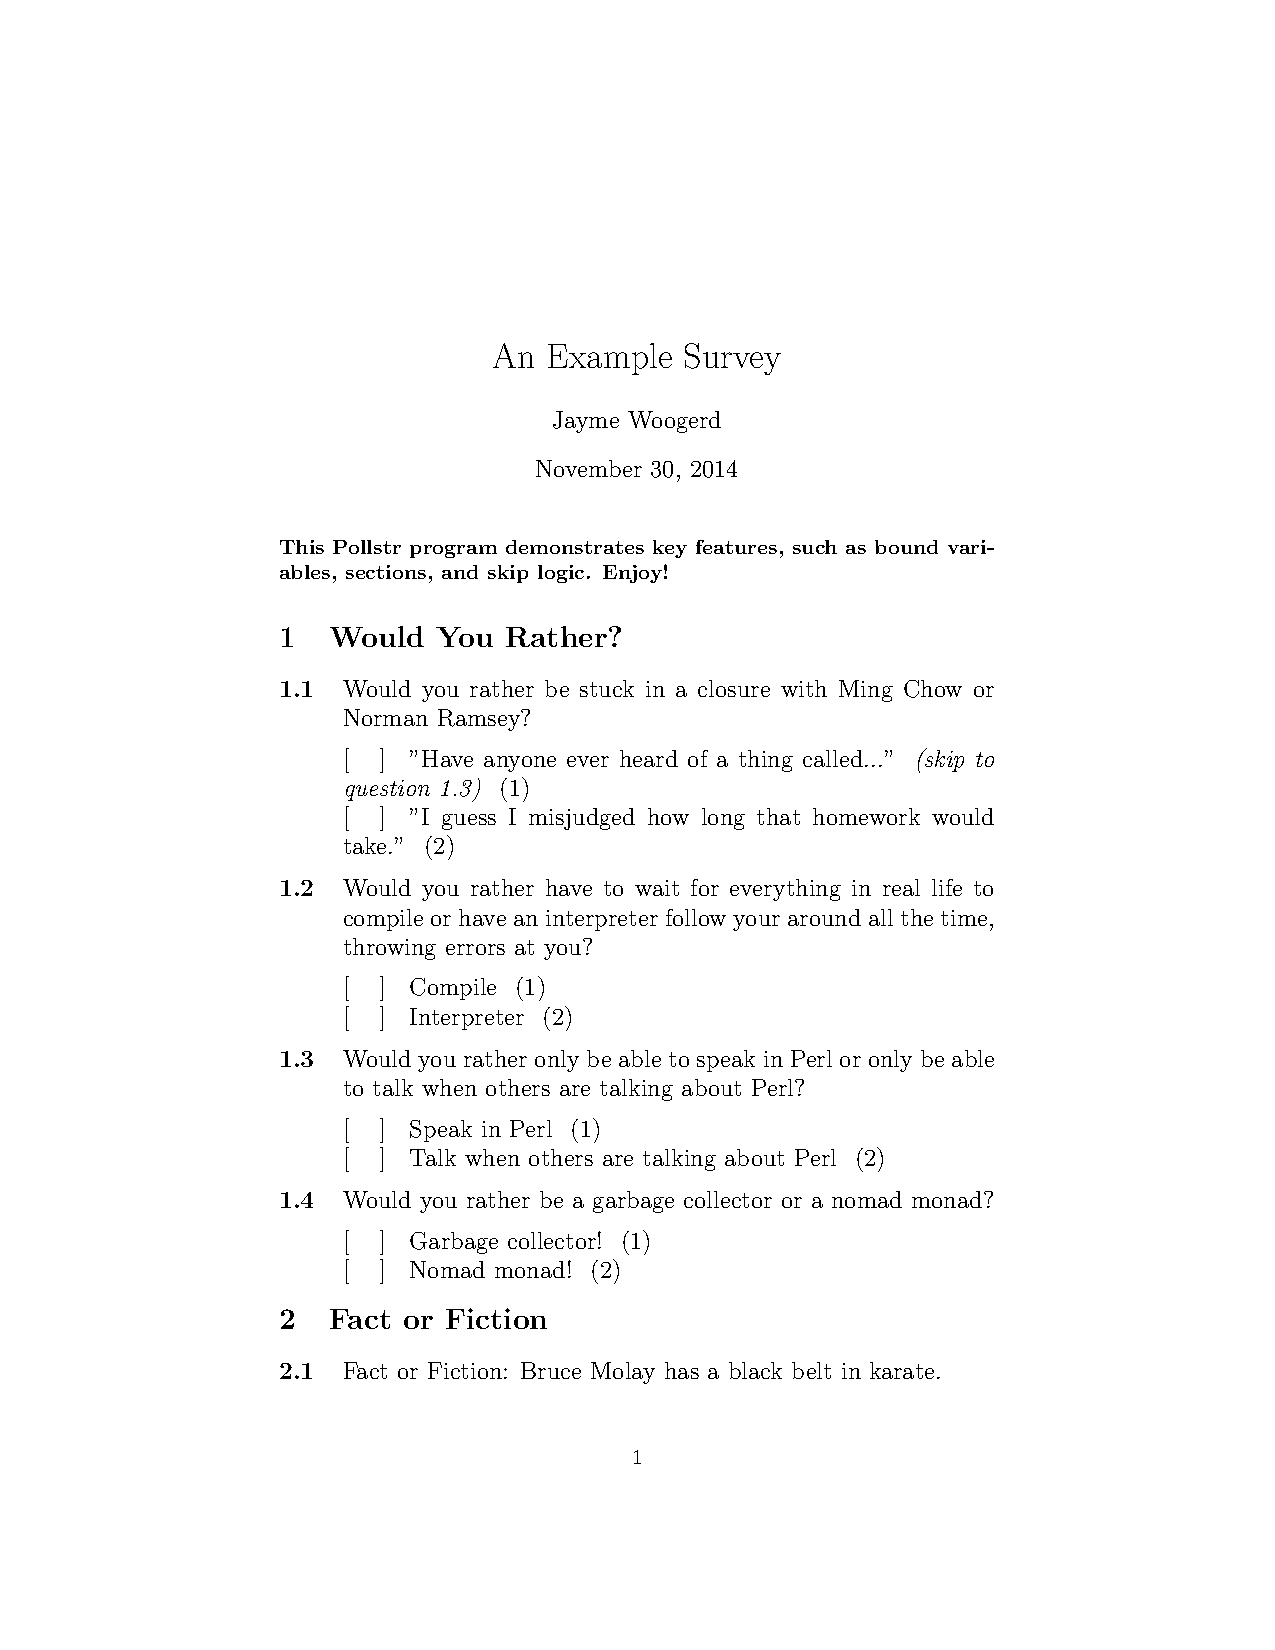
\includepdf[pages={-}]{demo.pdf}
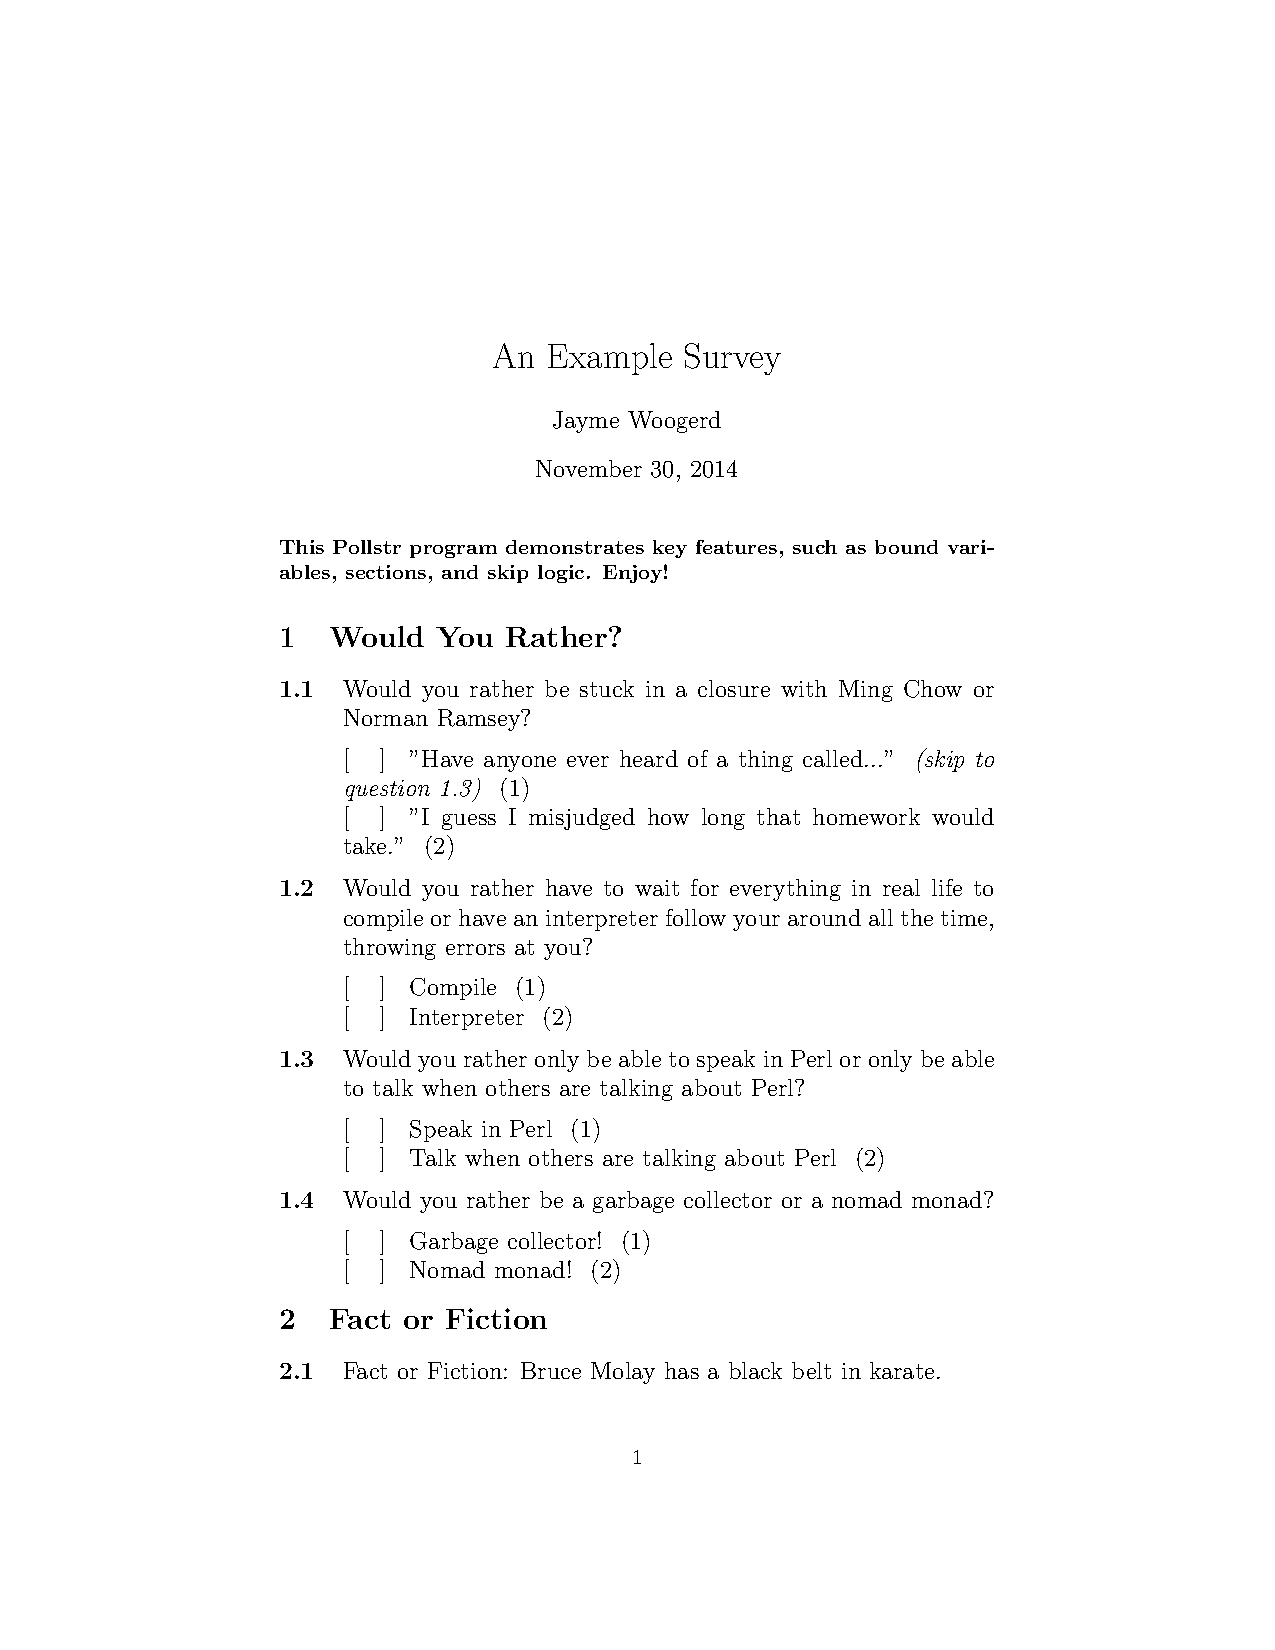
\includepdf[pages=1,pagecommand={},offset=-2.5cm -3cm]{demo.pdf}
\includepdf[pages=2,pagecommand={},offset=2.5cm -3cm]{demo.pdf}

\newpage
\begin{lstlisting}
{
    "sections": [
        {
            "items": [
                {
                    "skips": {
                        "resp": [
                            "\"Have anyone ever heard of a thing called...\""
                        ],
                        "to": "Q3"
                    },
                    "response": [
                        "\"Have anyone ever heard of a thing called...\"",
                        "\"I guess I misjudged how long that homework would take.\""
                    ],
                    "id": "Q1",
                    "question": "Would you rather be stuck in a closure with Ming Chow or Norman Ramsey?"
                },
                {
                    "response": [
                        "Compile",
                        "Interpreter"
                    ],
                    "id": "Q2",
                    "question": "Would you rather have to wait for everything in real life to compile or have an interpreter follow your around all the time, throwing errors at you?"
                },
                {
                    "response": [
                        "Speak in Perl",
                        "Talk when others are talking about Perl"
                    ],
                    "id": "Q3",
                    "question": "Would you rather only be able to speak in Perl or only be able to talk when others are talking about Perl? "
                },
                {
                    "response": [
                        "Garbage collector!",
                        "Nomad monad!"
                    ],
                    "id": "Q4",
                    "question": "Would you rather be a garbage collector or a nomad monad?"
                }
            ],
            "title": "Would You Rather?"
        },
        {
            "items": [
                {
                    "response": [
                        "Fact",
                        "Fiction"
                    ],
                    "id": "Q5",
                    "question": "Fact or Fiction: Bruce Molay has a black belt in karate."
                },
                {
                    "response": [
                        "Fact",
                        "Fiction"
                    ],
                    "id": "Q11",
                    "question": "Fact or Fiction: Sam Guyer is is a licensed airplane pilot."
                }
            ],
            "title": "Fact or Fiction"
        }
    ],
    "meta": {
        "author": "Jayme Woogerd",
        "title": "An Example Survey",
        "description": "This Pollstr program demonstrates key features, such as bound variables, sections, and skip logic. Enjoy!"
    }
}
\end{lstlisting}

\end{document}
